
\documentclass[preprint,12pt]{elsarticle}
\usepackage{adjustbox}
\usepackage{amssymb}
\usepackage{mathrsfs}
\usepackage{bm}

\journal{Information Sciences}
\usepackage{amsmath}
\usepackage{algorithmic}
\usepackage{url}
\usepackage{color,soul}
\soulregister\cite7
\soulregister\ref7
\soulregister\mathbf7
\usepackage{caption,subcaption}
\usepackage{ulem}
\usepackage{xcolor}
\usepackage{booktabs}
\setstcolor{red} 
\begin{document}
\begin{frontmatter}


\title{Attention-Based Bidirectional GRU Networks for Efficient HTTPS Traffic Classification}


\tnotetext[t1]{This work is supported by the National Key R\&D Program of China (Grant No. 2017YFB0801801), Strategic Priority Research Program of the Chinese Academy of Sciences (Grant No. XDC02070200), Strategic Priority Research Program of the Chinese Academy of Sciences (Grant No. XDC02060400), and the CNTC (China National Tobacco Corporation) Science and Technology Major Project under Grant No. 110201801020 (SJ-02).}


\author[1,2]{Xun Liu}
%\ead{liuxun@iie.ac.cn}

\author[1]{Junling You
\corref{cor1}}
\cortext[cor1]{Corresponding author}
%\ead{youjunling@iie.ac.cn}

\author[3]{Yulei Wu
\corref{cor1}}
%\ead[url]{www.stmdocs.in}
%\ead{Y.L.Wu@exeter.ac.uk}

\author[1]{Tong Li}
%\ead{litong@iie.ac.cn}

\author[1]{Liangxiong Li}
%\ead{liliangxiong@iie.ac.cn}

\author[1,2]{Zheyuan Zhang}
%\ead{zhangzheyuan@iie.ac.cn}

\author[1,2]{Jingguo Ge}
%\ead{gejingguo@iie.ac.cn}






\address[1]{Institute of Information Engineering, Chinese Academy of Sciences, Beijing, China}
\address[2]{School of Cyber Security, University of Chinese Academy of Sciences, Beijing, China}
\address[3]{College of Engineering, Mathematics and Physical Sciences, University of Exeter, Exeter, EX4 4QF, UK}






\begin{abstract}
%% Text of abstract
Distributed and pervasive web services have become a major platform for sharing information. However, the hypertext transfer protocol secure (HTTPS), which is a crucial web encryption technology for protecting the information security of users, creates a supervisory burden for network management (e.g., quality-of-service guarantees and traffic engineering). Identifying various types of encrypted traffic is crucial for cyber security and network management. In this paper, we propose a novel deep learning model called BGRUA to identify the web services running on HTTPS connections accurately. BGRUA utilizes a bidirectional gated recurrent unit (GRU) and attention mechanism to improve the accuracy of HTTPS traffic classification. The bidirectional GRU is used to extract the forward and backward features of the byte sequences in a session. The attention mechanism is adopted to assign weights to features according to their contributions to classification. 
%The idea of transfer learning is adopted to get the model re-trained quickly for the newly collected dataset. 
Additionally, we investigate the effects of different hyperparameters on the performance of BGRUA and present a set of optimal values that can serve as a basis for future relevant studies. Comparisons to existing methods based on three typical datasets demonstrate that BGRUA outperforms state-of-the-art encrypted traffic classification approaches in terms of accuracy, precision, recall, and F1-score.

\end{abstract}


\begin{keyword}
Encrypted traffic classification \sep HTTPS \sep Transfer learning \sep Bidirectional gated recurrent unit \sep Attention mechanism 
\end{keyword}
\end{frontmatter}





%% main text
\section{Introduction}
Based on the rapid development of web technologies, the number of different types of web applications has increased dramatically. Such applications include e-commerce \cite{Kenli2}, online banking, and instant messaging. The distributed and pervasive nature of web services is of particular importance for people who wish to share and receive information in their daily lives \cite{Kenli1}. Although web applications are a major driving force in modern society, they have introduced many security issues that cannot be ignored \cite{shbair2015efficiently}. In the early years of development, the mainstream protocol for web services was the hypertext transfer protocol (HTTP). Because the data handled by web services are transmitted in plaintext, they are naturally fragile and vulnerable. To protect the information and privacy of users, web services now use the secure HTTP (HTTPS) protocol for data transmission, which encapsulates the HTTP in transport-layer security (TLS) tunnels for information encryption \cite{naylor2014cost}.

Traffic analysis is an important tool for network management tasks \cite{DaiHN}, such as congestion control and quality-of-service guarantees \cite{shbair2017service}. However, HTTPS encryption introduces significant challenges for efficient traffic analysis.
Encrypted traffic classification is a crucial task in the field of traffic supervision and analysis. The server name indication (SNI) field carried during the plaintext transmission phase of a TLS connection is an important element that can be used to classify HTTPS services. An SNI-based firewall maintains a blacklist to block unsafe HTTPS domains. The authors of \cite{shbair2015efficiently} verified that if an SNI field is modified maliciously, it is possible to bypass a blacklist and establish a connection with a server. Many encrypted traffic classification methods have been proposed in recent years. Network traffic can be broadly divided into session-based and flow-based categories. The former contains bidirectional traffic and the latter contains one-directional traffic \cite{wang2017end}. 
%The representative datasets corresponding to these two categories will be selected to validate our model in this study.

According to the granularity of traffic classification, existing research can be divided into three categories \cite{shbair2016multi}: protocol-level, page-level, and service-level classification. Traditional protocol-level classification aims to identify different types of protocols, such as secure sockets layer (SSL), secure shell, and peer-to-peer (P2P) protocols \cite{wang2014characterizing}. Page-level approaches attempt to classify specific web pages \cite{cheng1998traffic}. Such approaches operate at the page-level based on static content, which is not suitable for modern websites containing dynamic content (e.g., content obtained from content delivery networks). Service-level classification attempts to identify application types \cite{kim2015method}, allowing network managers to obtain accurate traffic type and service provider information. Consequently, service-level classification has become the mainstream method. 

From the perspective of classification methods, existing research can be roughly divided into four categories: port-based, deep packet inspection (DPI)-based, session-based, and packet-based research. Early internet applications typically used fixed port numbers, meaning traffic could be identified based on port numbers. However, dynamic port numbers are now widely used for web services \cite{alshammari2009machine}. Therefore, port-based methods are no longer effective.
DPI methods analyze the content of packets by using predefined patterns, such as keywords or regular expressions, as signatures to classify traffic types. These types of methods have encountered significant difficulties since the advent of encrypted traffic \cite{nguyen2008survey}. Session-based methods adopt statistical features and traditional machine learning algorithms (such as C4.5) for classification. Their performance depends on feature selection \cite{velan2015survey}, which is a complicated and time-consuming process. 

In recent years, deep neural networks (DNNs) have seen rapid development for computer vision and natural language processing tasks.
DNNs possess excellent capabilities for feature extraction and can learn features via training instead of manual selection. Packet-based approaches that use neural networks to perform traffic classification have attracted significant attention from both academia and industry. However, there are still two major problems that significantly affect the performance of traffic classification. First, traffic data easily becomes outdated (e.g., upgraded application versions). Therefore, the data obtained in one time period may not follow the same distribution in a later time period. Additionally, there is no single traffic dataset that can represent all situations. Therefore, it is significant to update models quickly based on existing data. Second, the efficiency of DNNs is an important indicator of the performance of traffic classification. A large number of parameters in a DNN model will reduce the efficiency of traffic classification. One way to solve this problem is the adoption of distributed computing (i.e., distributed model training) to overcome the performance bottleneck of a single machine \cite{Kenli3}\cite{caspmv:}. Another promising method is transfer learning, which can accelerate convergence when training a new model. Most existing models fail to address these two problems, which largely determine whether a packet-based deep learning method can be developed from academia to industry.

We propose a novel method called BGRUA, which is an HTTPS traffic classification approach based on a bidirectional gated recurrent unit (GRU) network and an attention mechanism. BGRUA learns the features of packets through forward and backward GRU operations. It uses an attention mechanism to assign greater weights to useful features for encrypted traffic classification.
The final types of HTTPS services are classified using a fully connected softmax layer. To improve the efficiency of model training on different datasets, we introduce the concept of transfer learning to the field of traffic classification. For newly arriving traffic, our model only needs to adjust the fully connected layer to achieve rapid model convergence. We validated the accuracy of BGRUA on three datasets. Two of these datasets are open HTTPS datasets and the third is a dataset collected from the backbone of the China Science and Technology Network (CSTNET). Experimental results demonstrate that BGRUA outperforms state-of-the-art baselines. Additionally, instead of training models in new environments from scratch, BGRUA can be trained on a new dataset very quickly through transfer learning. The main contributions of this paper can be summarized as follows:

\begin{itemize}
\setlength{\itemsep}{0pt}
\setlength{\parsep}{0pt}
\setlength{\parskip}{0pt}
\item HTTPS traffic encryption hinders effective network supervision. In this paper, an original and novel framework is proposed to classify HTTPS services accurately without decrypting communication contents. The byte sequences of an HTTPS packet correspond to specific fields of a protocol and contain rich distinctive features. We designed a bidirectional GRU network to learn deep information from byte sequences automatically to facilitate classification. Traditional traffic classification methods assign the same weight to all features, which is not conducive to the extraction of important features. We combine a bidirectional GRU network with an attention mechanism to allow our model to focus on useful features that can contribute to effective traffic classification.

%
\item Encrypted traffic classification has strict requirements in terms of efficiency for real-world application scenarios. However, existing deep learning models are too time consuming to satisfy the requirements of real-time analysis. The proposed BGRUA not only improves the accuracy of traffic classification, but also reduces the number of parameters (i.e., weights) by a factor of seven compared to state-of-the-art models. This demonstrates that our method is more efficient for traffic classification.

%
\item Traditional classification models are only trained and evaluated on specific offline datasets, meaning they ignore the generation of new traffic and updated application versions. We introduce the concept of transfer learning into encrypted traffic classification. According to the diverse nature of traffic types and application versions in real network environments, BGRUA can be trained based on current knowledge to achieve rapid convergence. Experimental results demonstrate that the training speed on a new dataset is more than twice as fast as that of a model trained from scratch. 

\end{itemize}

The remainder of this paper is organized as follows. Section 2 introduces the background of the HTTPS. Section 3 discusses related work. Section 4 details the proposed model, including the data preprocessing layer, bidirectional GRU layer, attention layer, and transfer learning layer. Section 5 presents experimental results and performance analysis. Finally, we conclude this paper in Section 6.

\section{HTTPS Background}
The HTTPS guarantees secure communications for web services by wrapping the original HTTP in a secure TLS/SSL protocol. The TLS protocol aims to facilitate communication confidentiality and data integrity between two or more communicating applications. This protocol consists of two layers: a TLS handshake protocol and TLS record protocol. A TLS handshake occurs when a user retrieves information from an HTTPS website and the browser starts to query the server of that website. During the TLS handshake phase, communication parties exchange messages to confirm and verify each other and negotiate encryption algorithms. The TLS record protocol is used to encapsulate higher-level protocols. It is responsible for breaking down data from the application layer into fixed-length encrypted chunks. The record protocol also provides data integrity using message authentication codes, which are calculated based on an integrity key. The TLS handshake phase can summarized as follows.

As shown in Figure \ref{fig1}, the handshake protocol is of great importance because it is responsible for various configurations, such as cipher suite negotiation, authentication, and session key exchange. It can be divided into the following phases:

\begin{enumerate}
\item
A TLS handshake begins with a ``ClientHello'' message. In this message, the client sends a supported cipher suite, which is a series of cryptographic algorithms used to establish a secure communication connection. This message also carries the SNI field and a random number.
\item
The server responds with a ``ServerHello" message. This message includes the cipher suite selected by the server from the list provided by the client. The server also sends a certificate with a session ID and a random number.
\item
When the client verifies the certificate sent by the server, it sends a random byte string, also known as a ``Pre-Master Secret", and encrypts the string using the public key from the certificate.
\item
The communicating parties then generate a master key and session keys, which are used for symmetric encryption.
\item
The parties then exchange a ``ChangeCipherSpec" message and switch to symmetric encryption. The TLS handshake is concluded by sending a ``Finished" message.
\end{enumerate}

\begin{figure}[t]
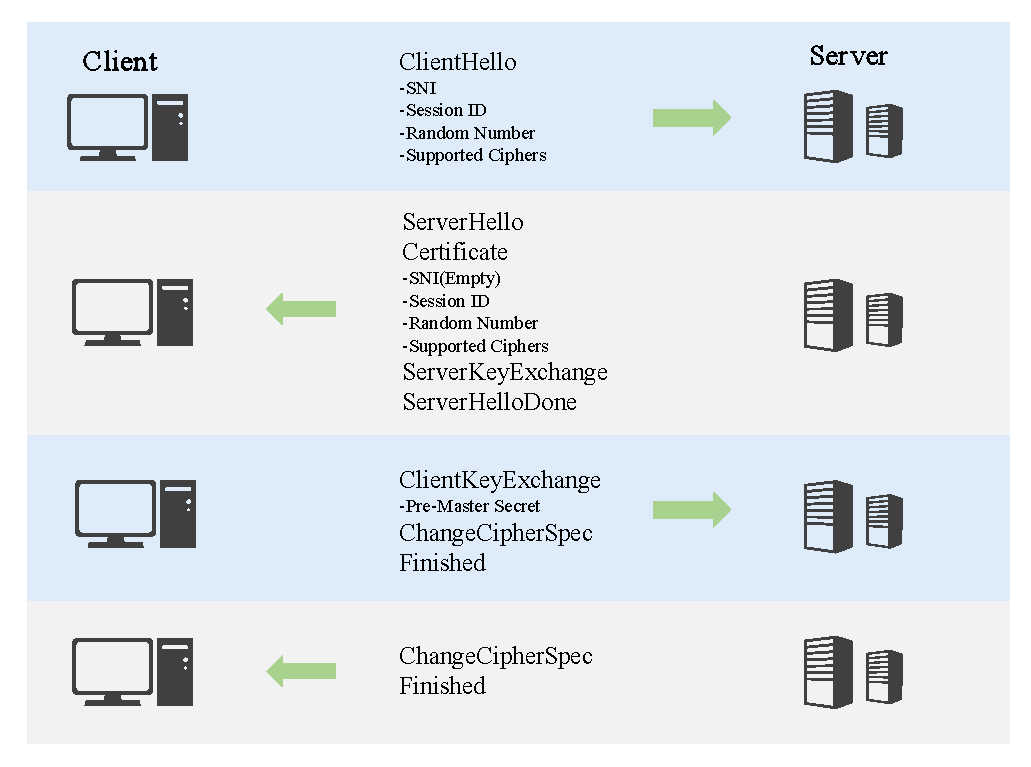
\includegraphics[width=\textwidth]{TLShandshake.eps}
\caption{The TLS Handshake process.} \label{fig1}
\end{figure}





\section{Related Work}
Recall that port-based and DPI-based methods are no longer applicable to encrypted traffic classification. Therefore, session-based and packet-based methods have become the mainstream methods. Previous studies on these two types of methods are summarized in Tables \ref{tab:my-table1} and \ref{tab:my-table2}, respectively. We briefly discuss these existing studies below. 

\subsection{Encrypted traffic classification}

\subsubsection{Session-based methods}

\begin{figure}[!t]
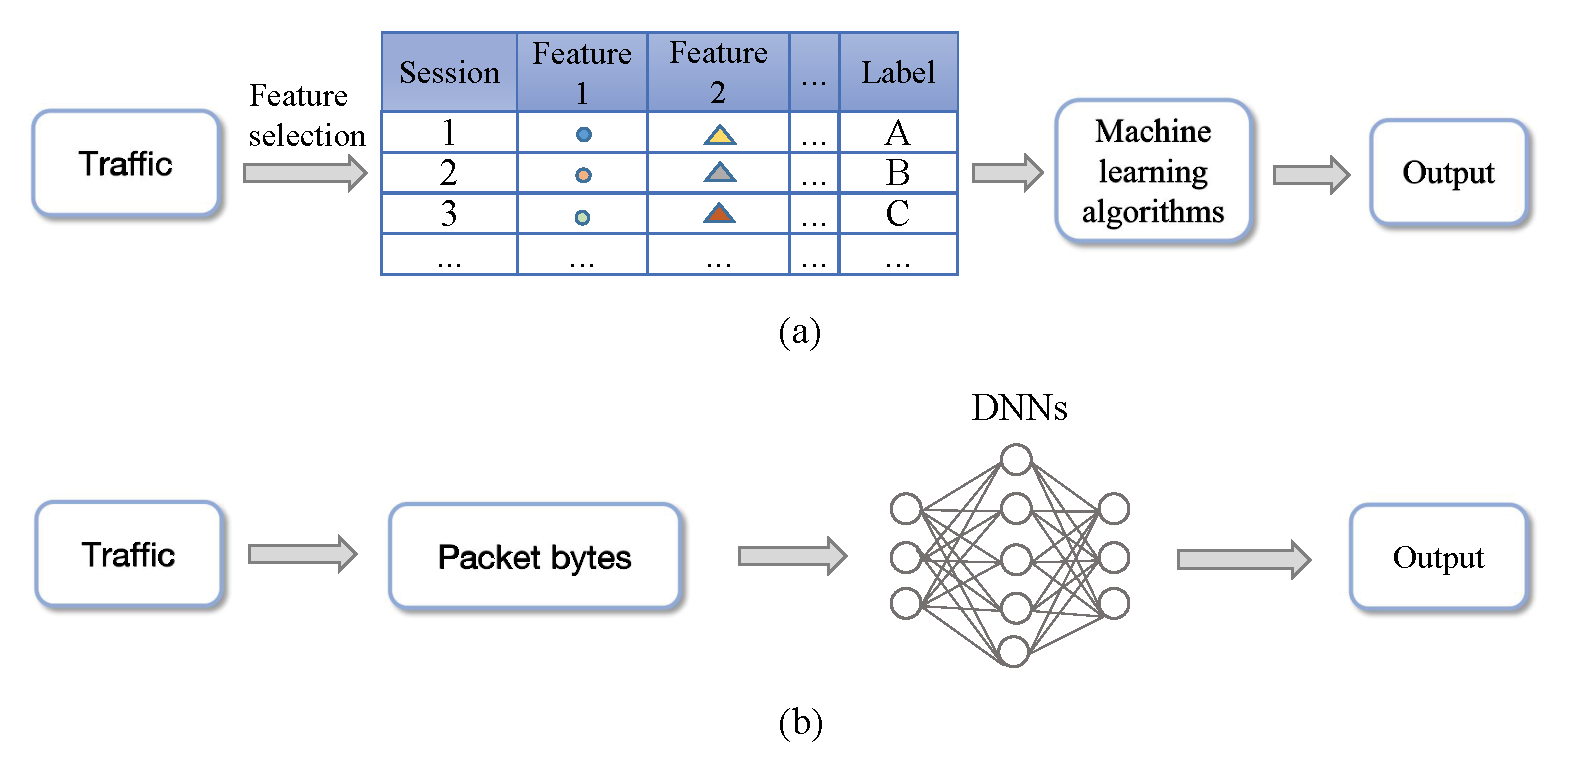
\includegraphics[width=\textwidth]{compare.eps}
\caption{Comparison of two common classification methods for encrypted traffic: (a) session-based methods and (b) packet-based methods.} \label{fig2}
\end{figure}


The general procedure for session-based methods is illustrated in Figure~\ref{fig2}(a). Session-based methods require the manual extraction of session features. These features are then used as inputs for a classifier. They are also used to train classification algorithms, such as a support vector machine (SVM), C4.5, or a random forest. Notably, it is not necessarily true that a greater number of features will result in better performance. Redundant and useless features increase computational complexity and reduce the accuracy of a classifier. Moore et al. \cite{moore2013discriminators} discussed 249 session-based and packet-based features, including packet size, packet interval, packet numbers in a session, and session duration. Subsequent traffic classification works have largely focused on combinations of these 249 features.

Session-based methods for traffic classification tasks can be divided into supervised learning, semi-supervised learning, and unsupervised learning methods. In supervised learning methods, encrypted sessions are labeled according to traffic categories and classifiers classify sessions based on a set of predefined categories. Supervised learning methods have developed rapidly in the field of traffic classification. As early as 2005, the authors of \cite{Moore:2005} proposed a Naive Bayes method to identify traffic and achieved an accuracy of 95\%. Sun et al. \cite{Sun} proposed a hybrid method for classifying encrypted traffic. In this method, the SSL/TLS protocol was first recognized using a signature matching method. A Naive Bayes machine learning algorithm was then applied to identify encrypted applications under the SSL/TLS protocol. Okada et al. \cite{okada2011comparisons} proposed the estimated features method (EFM) and evaluated the performance of three supervised learning algorithms (SVM, Naive Bayes, and C4.5). Experimental results demonstrated that the EFM with an SVM can achieve an overall accuracy of 97.2\% for encrypted traffic. The authors of \cite{ALSHAMMARI201577} investigated the performance of C5.0, AdaBoost, and a genetic programming (GP) algorithm for identifying voice over IP (VoIP) traffic. Datasets for experiments were captured on their campus networks (Univ2017 and Univ2019) and in their lab. They concluded that applying suitable sampling and machine learning methods is of great significance for classifying VoIP traffic.
Shbair et al. \cite{shbair2016multi} defined a new set of statistical features and trained a multi-level random forest classifier to identify services in HTTPS traffic. This method obtained a high accuracy of 93.10\%. 


In contrast, unsupervised learning methods are able to discover traffic patterns without predefined labels. Traffic patterns with similar characteristics tend to converge to the same cluster. Therefore, unsupervised learning can discover and process unknown traffic patterns. McGregor et al. \cite{McGregor} used the expectation maximization (EM) algorithm to verify that unsupervised learning can effectively evaluate cluster traffic. 
Erman et al. \cite{ErmanAM06} evaluated three classic clustering algorithms called AutoClass, DBSCAN, and K-Means.
The performances of these three algorithms were compared through various experiments.
Liu et al. \cite{LiuL11b} applied fuzzy C-means clustering technology to automatic P2P traffic classification. Furthermore, they modified the objective function and distance function to decrease computational complexity. Bernaille et al. \cite{BernailleTS06} selected the size and direction of the first few packets in a flow as features. They evaluated the performance of three clustering algorithms: K-means, a Gaussian mixture model, and spectral clustering. Finamore et al.\cite{Finamore} presented a modified K-means algorithm to determine numbers of traffic clusters automatically. They selected the Kiss signatures obtained from packet payloads as features. Experimental results demonstrated the effectiveness of their clustering algorithm.

 
In semi-supervised learning, a set of labeled traffic is used to map clusters to real applications. Erman et al. \cite{Erman:2007} used the K-Means method to cluster traffic, where labeled data in the clusters were used to identify cluster categories according to the majority principle. However, the results of the K-Means algorithm are sensitive to the selection of initial cluster centers and may converge to local optima. The authors for \cite{Liu11} considered the clustering problem as an optimization problem and applied particle swarm optimization (PSO) to identify the optimal centers of clusters. The goal of PSO is to maximize the distance between clusters and minimize intra-cluster distance. To improve classification performance when few labeled training samples are available, Zhang et al. \cite{DBLP:journals/ijsn/ZhangCXZ12} proposed the incorporation of flow correlation into both the training and testing stages.

\begin{table}[h]
%\renewcommand\arraystretch{1.2}
\setlength{\abovecaptionskip}{0pt}
\setlength{\parskip}{3ex}
\centering
\caption{Summary of existing session-based methods.}
\label{tab:my-table1}
\resizebox{\textwidth}{!}{%
\begin{tabular}{lllll}
\toprule
\textbf{Ref. ID} & \textbf{Features}                                                                               & \textbf{Classifiers}                                                                               & \textbf{Dataset}                                                                       & \textbf{Results}                                                                                      \\ \hline
{}\cite{shbair2016multi}{}          & \begin{tabular}[c]{@{}l@{}}Average size, \\ 25/50/75th \\ percentile size, etc.\end{tabular}    & \begin{tabular}[c]{@{}l@{}}Multi-level random \\ forest\end{tabular}                               & \begin{tabular}[c]{@{}l@{}}Captured on their \\ lab\end{tabular}                       & Accuracy: 93.1\%                                                                                      \\
{}\cite{Moore:2005}{}         & \begin{tabular}[c]{@{}l@{}}Session duration, \\ TCP Port, etc.\end{tabular}                     & Naive Bayes                                                                                        & Private datasets                                                                       & Accuracy: 95\%                                                                                        \\
{}\cite{Sun}{}         & \begin{tabular}[c]{@{}l@{}}Packet length and \\ arrival time, etc.\end{tabular}                 & \begin{tabular}[c]{@{}l@{}}Signature-based and \\ Bayesian method\end{tabular}                     & \begin{tabular}[c]{@{}l@{}}Private and public \\ datasets\end{tabular}                 & \begin{tabular}[c]{@{}l@{}}F-score for protocols \\ identification:94.52\%\end{tabular}               \\
{}\cite{okada2011comparisons}{}         & \begin{tabular}[c]{@{}l@{}}Packet size and \\ inter-arrival time, etc.\end{tabular}             & \begin{tabular}[c]{@{}l@{}}Estimated features \\ method\end{tabular}                               & \begin{tabular}[c]{@{}l@{}}Captured on two major \\ ISPs in Japan\end{tabular}         & \begin{tabular}[c]{@{}l@{}}Accuracy: 97.2\% (using \\ SVM)\end{tabular}                               \\
{}\cite{ALSHAMMARI201577}{}         & \begin{tabular}[c]{@{}l@{}}Session-based \\ feature set\end{tabular}                            & \begin{tabular}[c]{@{}l@{}}C5.0, AdaBoost and \\ GP\end{tabular}                                   & Univ2017, Univ2019                                                                     & Evaluated three algorithms                                                                            \\
{}\cite{McGregor}{}         & \begin{tabular}[c]{@{}l@{}}Packet size statistics,\\ inter-arrival statistics, etc.\end{tabular} & EM algorithm                                                                                       & \begin{tabular}[c]{@{}l@{}}From the University of \\ Auckland and Waikato\end{tabular} & This method is very effective                                                                         \\
{}\cite{ErmanAM06}{}         & Transport layer statistics                                                                      & \begin{tabular}[c]{@{}l@{}}AutoClass, K-Means,\\ DBSCAN\end{tabular}                               & \begin{tabular}[c]{@{}l@{}}1. Auckland IV\\ 2. Collected privately\end{tabular}        & Compared three algorithms                                                                             \\
{}\cite{LiuL11b}{}         & \begin{tabular}[c]{@{}l@{}}Session and packet \\ statistics\end{tabular}                        & Fuzzy C-Means                                                                                      & \begin{tabular}[c]{@{}l@{}}Captured in an \\ empirical platform\end{tabular}           & Real-time and efficient                                                                               \\
{}\cite{BernailleTS06}{}         & \begin{tabular}[c]{@{}l@{}}Size and direction of \\ first few packets\end{tabular}              & \begin{tabular}[c]{@{}l@{}}K-Means, Gaussian,\\  Mixture model,\\ Spectral clustering\end{tabular} & \begin{tabular}[c]{@{}l@{}}Collected on 8 \\ different networks\end{tabular}           & Accuracy: over 90\%                                                                                   \\
{}\cite{Finamore}{}         & Kiss signatures                                                                                 & Modified K-Means                                                                                   & \begin{tabular}[c]{@{}l@{}}ISP-Trace and \\ P2PTV-Trace\end{tabular}                   & Accuracy: above 95\%                                                                                  \\
{}\cite{Erman:2007}{}         & Attribute vectors                                                                               & K-Means                                                                                            & Private dataset                                                                        & \begin{tabular}[c]{@{}l@{}}A fast and accurate \\ classifiers with small \\ labeled data\end{tabular} \\
{}\cite{Liu11}{}         & Three P2P traffic metrics                                                                       & PSO                                                                                                & Established manually                                                                   & High precision                                                                                        \\
{}\cite{DBLP:journals/ijsn/ZhangCXZ12}{}         & \begin{tabular}[c]{@{}l@{}}Session level \\ statistical properties\end{tabular}                 & \begin{tabular}[c]{@{}l@{}}Incorporate flow \\ correlation\end{tabular}                            & \begin{tabular}[c]{@{}l@{}}Public real-world \\ traffic dataset\end{tabular}           & \begin{tabular}[c]{@{}l@{}}Outperforms the \\ state-of-the-art methods\end{tabular}    \\
\bottomrule
\end{tabular}%
}
\end{table}


\subsubsection{Packet-based methods}

As shown in Figure \ref{fig2}(b), unlike session-based methods, packet-based approaches eliminate the need for manual feature selection and use packet bytes directly. Preprocessed packet bytes are fed into deep learning models for feature extraction. A softmax classifier is typically used to calculate the probability value of each category. Packet-based methods have attracted the attention of researchers for several years. Wang et al. \cite{wang2015applications} selected the first 1000 payload bytes in a session as features and mined optimal features using artificial neural networks (ANNs). Their classifier classified sessions with a probability of less than 0.8 for unknown traffic. Lotfollahi et al. \cite{lotfollahi2017deep} designed a framework called Deep Packet. They used 1500 byte vectors as the inputs for Deep Packet, which combines a stacked autoencoder with CNNs to classify network traffic. Deep Packet achieved a recall of 0.98 on an application classification task. The authors of \cite{wang2017end} trained a 1D CNN model using the first 784 bytes of each flow or session. Their 1D CNN achieved outstanding performance compared to the traditional C4.5 algorithm. Wang et al. \cite{wang2017malware} applied deep learning methods to malware traffic classification. They transformed packet bytes into 2D images and applied a 2D CNN to perform classification. This approach only uses the spatial features of traffic and ignores temporal features. Zou et al. \cite{zou2018encrypted} extracted the spatial features inside packets using a 2D CNN and learned the temporal features contained in flows using long short-term memory (LSTM). They evaluated their model on the ISCX VPN-nonVPN traffic dataset. The results demonstrated that this model can improve the accuracy of traffic classification by up to 6\% compared to a 1D CNN model. 

Regarding unsupervised learning, Zhao et al. \cite{DBLP:conf/ict/Zhao0S19} proposed a novel unknown traffic clustering scheme based on n-gram embeddings and DNNs. They characterized traffic payloads using different lengths of n-gram embeddings and extracted features using a deep autoencoder. They achieved an average clustering accuracy rate of 97.35\%. Zhang et al. \cite{iccS/Zhang} proposed the DePCK method for classifying unknown traffic based on a deep autoencoder and modified pairwise constrained PCKMeans algorithm. To improve performance with few labeled samples, Iliyasu et al. \cite{Iliyasu} proposed a semi-supervised learning approach based on a deep convolutional generative adversarial network (DCGAN). They used samples generated by the DCGAN and unlabeled traffic to improve classifier performance.

\begin{table}[]
%\renewcommand\arraystretch{1.2}
\setlength{\abovecaptionskip}{0pt}
\setlength{\parskip}{3ex}
\centering
\caption{A summary of existing packet-based methods.}
\label{tab:my-table2}
\resizebox{\textwidth}{!}{%
\begin{tabular}{lllll}
\toprule
\textbf{Ref. ID}  & \textbf{Features}                                                                                        & \textbf{Classifiers}                                                                    & \textbf{Dataset}                                                                                & \textbf{Results}                                                                                              \\ \hline
{}\cite{wang2017end}{}  & The first 784 bytes                                                                             & 1D-CNN                                                                         & ISCX VPN-nonVPN                                                                        & \begin{tabular}[c]{@{}l@{}}Better than the C4.5 \\ algorithm\end{tabular}                            \\
{}\cite{wang2015applications}{} & \begin{tabular}[c]{@{}l@{}}The first 1000 \\ payload bytes\end{tabular}                         & ANN                                                                            & \begin{tabular}[c]{@{}l@{}}From the internal \\ network\end{tabular}                   & The model works very well                                                                            \\
{}\cite{lotfollahi2017deep}{} & 1500 payload bytes                                                                              & SAE, CNN                                                                       & ISCX VPN-nonVPN                                                                        & Recall: 98\%                                                                                         \\
{}\cite{wang2017malware}{} & The first 784 bytes                                                                             & CNN                                                                            & USTC-TFC2016                                                                           & Average accuracy: 99.41\%                                                                            \\
{}\cite{zou2018encrypted}{} & \begin{tabular}[c]{@{}l@{}}First three 784 \\ packet bytes\end{tabular}                         & CNN-LSTM                                                                       & ISCX VPN-nonVPN                                                                        & \begin{tabular}[c]{@{}l@{}}Accuracy improves 6\% in \\ comparison with 1D-CNN\end{tabular}           \\
{}\cite{DBLP:conf/ict/Zhao0S19}{} & Packet bytes                                                                                    & \begin{tabular}[c]{@{}l@{}}Autoencoder, \\ K-Means\end{tabular}                & \begin{tabular}[c]{@{}l@{}}Collected from \\ campus network\end{tabular}               & \begin{tabular}[c]{@{}l@{}}Clustering purity rate: \\ about 97.35\%\end{tabular}                      \\
{}\cite{iccS/Zhang}{} & Deep Embedding                                                                                  & \begin{tabular}[c]{@{}l@{}}Deep Autoencoder, \\ PCKMeans\end{tabular}          & WIDE and ISP                                                                           & \begin{tabular}[c]{@{}l@{}}Clustering purity rate: \\ 94.81\% (ISP), 91.48\% \\ (WIDE)\end{tabular}  \\
{}\cite{Iliyasu}{} & \begin{tabular}[c]{@{}l@{}}Time-series properties \\ of packets\end{tabular}                    & DCGAN                                                                          & \begin{tabular}[c]{@{}l@{}}1. Self-collected QUIC\\ 2. ISCX VPN-NonVPN\end{tabular}    & \begin{tabular}[c]{@{}l@{}}Accuracy: 89\%(QUIC) \\ 78\%(ISCX)\end{tabular} \\  
\bottomrule
\end{tabular}%
}
\end{table}


\subsection{Transfer learning} Many session-based and packet-based methods perform well in cases where training data and testing data follow the same distribution. However, when a data distribution changes, most of these models must be retrained from scratch based on newly collected data \cite{weiss2016survey}. The purpose of transfer learning is to solve problems quickly and precisely based on previously learned knowledge. The concept of transfer learning was proposed in \cite{Caruana:95}. Since then, many researchers have devoted significant attention to this concept. Several studies have shown that transfer learning can increase the convergence speed of model training. In object classification tasks, transfer learning significantly reduces training time by approximately 92\% compared to a baseline method and reduces classification time by approximately 99\% \cite{Kawewong}. Lebedev et al. \cite{lebedev2014speeding} proposed a simple two-step approach to accelerating convolutional layers within a large CNN based on tensor decomposition and discriminative fine-tuning. The authors of \cite{Takano} accelerated the learning processes of reinforcement learning by incorporating transfer learning. Transfer learning has been successfully applied to text recognition \cite{wang2011heterogeneous}, recommendation systems, image processing \cite{Eaton} \cite{Kulis} \cite{Zhu}, software defect classification \cite{nam2015heterogeneous}, etc. However, transfer learning has received relatively little attention in the field of encrypted traffic classification. 

%***a new paragraph to emphasise the contribution of this paper, in contrast to the disadvantages of the existing studeis.***
In summary, traditional session-based methods require manual feature extraction, which is time consuming and inefficient. Some features can only be obtained when a session ends, such as the session duration and total number of packets in a session, making such methods inapplicable for real-time analysis. In existing deep learning methods, the numbers of parameters for different models are very large and calculation complexity is high. Additionally, existing models do not consider the performance degradation caused by changes in traffic distributions. Considering the disadvantages of existing methods, we propose a novel method that only requires the first three packets in a session to classify HTTPS traffic, instead of requiring all packets from a full session. The small number of parameters in our model significantly improves classification speed. By adopting the concept of transfer learning, our model can also converge quickly on newly collected data.






\setcounter{figure}{2}
\setcounter{table}{2}
\section{Proposed Model}
In this section, we present the framework of BGRUA. As shown in Figure~\ref{fig3}, the architecture of BGRUA consists of four layers: a data preprocessing layer, bidirectional GRU layer, attention layer, and transfer learning layer. Each of these layers is detailed in the following subsections.


%***this figure doesn't show data pre-processing layer clearly and transfer learning layer at all. Please improve.***
\begin{figure}[!t]
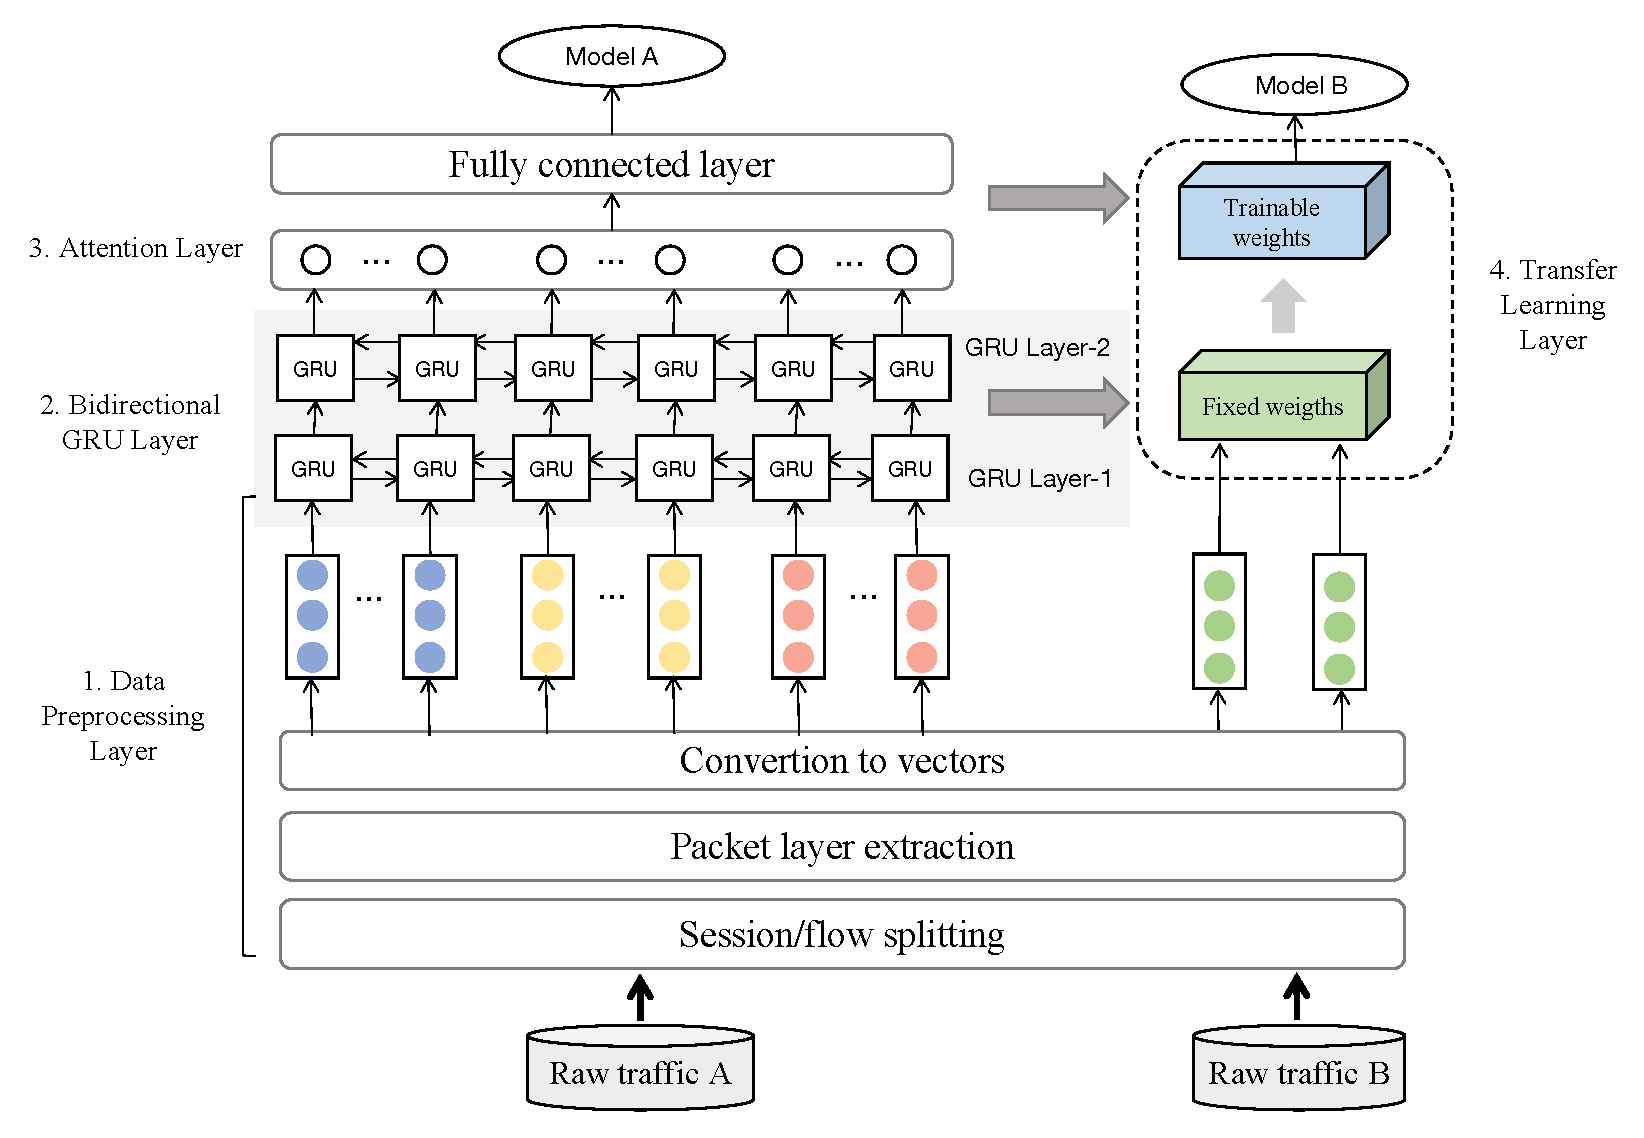
\includegraphics[width=\textwidth]{overview.eps}
\caption{Overview of the proposed BGRUA model.} \label{fig3}
\end{figure}

\subsection{Data Preprocessing Layer}
\noindent\textbf{Session/flow splitting.} 
Raw traffic data contains multiple .pcap files extracted from a network. These files must be split into sessions according to five-tuples (i.e., source IP, destination IP, source port, destination port, and transport-layer protocol). In this study, we conducted experiments on three datasets denoted as A, B, and C (see Section \ref{sec: datasets}). Datasets A and C contain full TLS sessions between a client and server, whereas Dataset B only includes flows originating from a client.


\noindent\textbf{Packet layer extraction.} 
Packet-based classification methods typically adopt packet payloads as the inputs for a neural network. A common practice is to select the first $P$ packets in a session, where each packet contains $B$ bytes. $P$ and $B$ are hyperparameters for neural network models and must be defined prior to model training. In this study, $P$ was set to three and $B$ was set to 900. In Section \ref{sec: model comparison and analysis}, we investigate the effects of the values of $P$ and $B$ on the performance of BGRUA. Specifically, we extract packet bytes starting from the transport layer and then perform truncation if the payload length exceeds 900 and padding with zeros if the payload length is less than 900. Additionally, we remove the SNI extension by replacing the corresponding bytes with zeros. This prevents our network from learning features by relying on the SNI field.  

\noindent\textbf{Conversion to vectors.} 
For each session, we obtain three consecutive 900 byte packages (i.e., a total of 2700 bytes). Each byte can be converted into an integer between 0 and 255. The inputs for the GRU networks are fixed-dimension vectors $\mathbf{x_t}$ at time step $t$. In our model, the dimension of $\mathbf{x_t}$ is 150, meaning vectors are formed from 150 byte packages. We can derive 18 vectors as follows:


\begin{equation}
    \mathbf{x_1} = b_1 \oplus b_2 \oplus ... \oplus b_{150},
\end{equation}
\begin{equation}
    \mathbf{x_2} = b_{151} \oplus b_{152} \oplus ... \oplus b_{300}
\end{equation}
\begin{center}
%\begin{equation*}
    ...
%\end{equation*}
\end{center}
\begin{equation}
    \mathbf{x_{18}} = b_{2551} \oplus b_{2552} \oplus ... \oplus b_{2700},
\end{equation}
where $\oplus$ is a concatenation operator and $b$ denotes a specific byte. The vector sequence $X = (\mathbf{x_1}, \mathbf{x_2},..., \mathbf{x_{18}} )$ is normalized to $[0, 1]$ by dividing 255 and is then fed into the bidirectional GRU networks for subsequent training and testing.

\begin{figure}[hbt]
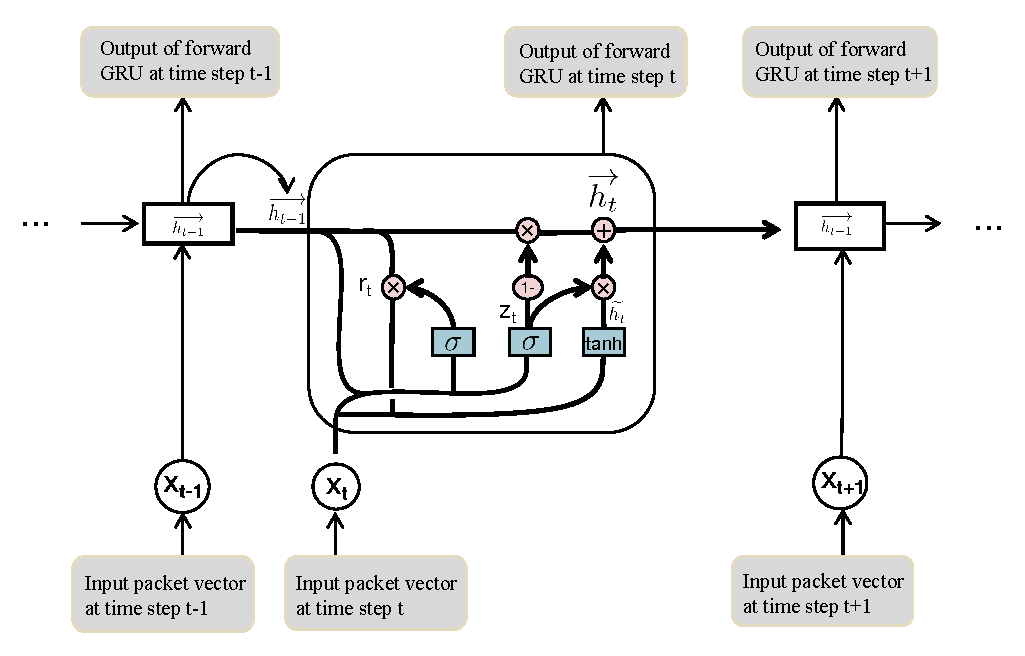
\includegraphics[width=\textwidth]{gru.eps}
\caption{Structure of the forward GRU at time step $t$.}\label{fig4}
\end{figure}


\subsection{Bidirectional GRU Layer} \label{sec: bidirectional_gru_layer}
Recurrent neural networks (RNNs) \cite{mikolov2010recurrent} have been successfully applied in many fields. Because they contain self-connected hidden layers, RNNs can use their internal states to process time-related sequences. The GRU is a variant of an RNN that can overcome the issues of vanishing gradients and gradient explosions in traditional RNNs. More importantly, a GRU can learn both long-term and short-term dependences, unlike a traditional RNN.

Our recurrent network consists of two bidirectional GRU layers (i.e., GRU layer-1 and GRU layer-2). As shown in Figure~\ref{fig3}, each layer consists of a forward GRU and a backward GRU. Each GRU includes an input layer and self-connected hidden layer. In BGRUA, all states in each GRU are initialized to zero, and the number of hidden units is set to 256. The forward GRU takes the sequences $X = (\mathbf{x_1}, \mathbf{x_2},..., \mathbf{x_{18}})$ generated by the data preprocessing layer as sequential inputs. As shown in Figure~\ref{fig4}, at a time step $t$ ($0 < t \leq 18$), the $t$-th vector $\mathbf{x_t}$ of $X$ is sent to the input layer of the forward GRU. The hidden layer combines $\mathbf{x_t}$ and the hidden state $\overrightarrow{h_{t-1}}$ at time step $t-1$ to perform a series of linear operations and activation operations. There are two gates in each GRU, namely an update gate $z_t$ and reset gate $r_t$. The gate $z_t$ controls how much previous information is retained in the current state and the gate $r_t$ determines how strongly irrelevant bytes sequences are ignored, thereby ensuring that important byte sequences are passed to the next step. All of the relationships in the forward GRU can be defined as follows:
 


\begin{equation}
    z_t = \sigma(W_z[\overrightarrow{h_{t-1}},\mathbf{x_t}]),
\end{equation}

\begin{equation}
    r_t = \sigma(W_r[\overrightarrow{h_{t-1}},\mathbf{x_t}]),
\end{equation}


\begin{equation}
    \tilde{h_t} = tanh(W[r_t \overrightarrow{h_{t-1}},\mathbf{x_t}]),
\end{equation}

\begin{equation}
    \overrightarrow{h_t} = (1-z_t) \overrightarrow{h_{t-1}} + z_t \tilde{h_t},
\end{equation}
where $\mathbf{x_t}$ and $\overrightarrow{h_{t-1}}$ are the same as above, and $W_z$, $W_r$, and $W$ are weight matrices. $\sigma$ represents the sigmoid activation function, which transforms the intermediate state into the range of $0-1$ to act as a gating signal. $\overrightarrow{h_t}$ indicates the hidden state at time step $t$.


The backward GRU takes the sequence $X$ in reverse as an input. At time step $t$, it performs a series of calculations similar to the forward GRU and obtains a hidden state $\overleftarrow{h_t}$, which is spliced with $\overrightarrow{h_t}$ to form the final output $h_t$, as indicated in Eq. (8). After the final time step, we have the final output $H = (h_1, h_2,...,h_{18})$ of GRU layer-1. This bidirectional GRU scheme can analyze the correlations of packet vectors and extract features more accurately and comprehensively through forward and backward propagation. To capture deeper information, $H$ is fed into GRU layer-2, which has the same structure as GRU layer-1. The output of GRU layer-2 is then used as the input for the attention layer.


\begin{equation}
    h_t = [\overrightarrow{h_t},\overleftarrow{h_t}]
\end{equation}



\subsection{Attention Layer}
Not all packet vectors contribute equally to the classification of HTTPS traffic. Therefore, greater attention should be assigned to more useful vectors. As shown in Figure~\ref{fig12}, the attention layer is utilized to learn a weight $\alpha{_{t}}$ for each hidden state $h_t$ obtained at time step \textit{t} by the bidirectional GRU layer-2. Because there are a total of 18 time steps, \textit{t} is an integer number in the range of [1,18]. The weighting vector $\bm{\alpha} = (\alpha{_1},\alpha{_2},...,\alpha{_{18}})$ is calculated with respect to the output sequence $H = (h_1, h_2,...,h_{18})$. The attention vector $\textbf{s}$ is computed as a weighted sum of these 18 hidden states as follows:


\begin{equation}
    \bm{s} = \sum_{t=1}^{18} \alpha{_t}h_t,
\end{equation}
where the weighting factors $\alpha{_t}$ are calculated as follows:
\begin{equation}
    \alpha{_t} = \frac{exp(u_t^{T}u_w)}{\sum_{t} exp(u_t^{T}u_w)},
\end{equation}
\begin{equation}
    u_t = tanh(W_wh_t + b_w),
\end{equation}
where $W_w$ and $u_w$ denote weight matrices and $b_w$ denotes the bias. The outputs of the attention layer are sent to the fully connected layer. The $c$-way softmax function generates a probability over $c$ class labels. The variable $c$ is the number of traffic classes in the dataset.

\begin{figure}[]
\centerline{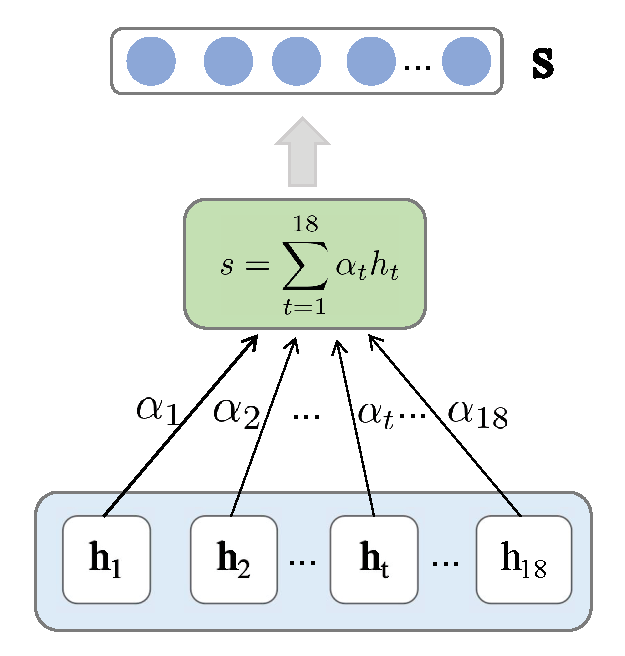
\includegraphics[width=6.5cm,height=6.5cm]{attention_layer.eps}}
\caption{Structure of the attention layer.}\label{fig12}
\end{figure}
\subsection{Transfer Learning Layer}

HTTPS traffic easily becomes outdated based on upgrades to protocol versions or web application versions. Therefore, the data distribution in one time period may change in a later time period. In a real-world network environment, there are many types of traffic and new traffic is frequently created. Training a model from scratch is time consuming and inefficient. Therefore, our transfer learning layer is designed to apply previously learned knowledge to solve new problems more quickly and accurately.

As shown in Figure~\ref{fig3}, following the data preprocessing layer, bidirectional GRU layer, and attention layer, a well-trained model can be obtained for the source domain $D_S = (x_i, y_i)$, where $x_i$ is the packet vector of the $i$-th session and $y_i$ is the corresponding label. We obtain a function $f_s$ through training and use it to predict HTTPS services. Given a newly collected dataset from the target domain $D_T$, the transfer learning layer uses the existing knowledge $D_S$ to assist $D_T$ to construct a new prediction function $f_t$ rapidly. To achieve rapid reconstruction, the structure of the transfer learning layer only retrains the weights of the fully connected layer. This is because more general features can be extracted in the lower layers of a network and can be transferred to other tasks. However, features become more task specific in nature in higher layers \cite{KAYA201920}. 

Based on the four layers described above, BGRUA can not only be applied to specific classification tasks, but can also reuse pre-trained models for similar new tasks.






\section{Experimental Results and Evaluation}
In this section, we evaluate the performance of the proposed BGRUA model. All experiments were performed on a Dell R720 machine with an Ubuntu operating system. TensorFlow was used as a software framework. Table~\ref{tab3} provides a detailed description of our experimental configuration. During training, the mini-batch size is 32 and the cost function is cross entropy. We use the Adam optimizer with an initial learning rate of 1e-3 and a decay rate of 0.96 in every epoch. The training procedure runs for 20 epochs.


\begin{table}[]
\centering
\caption{Experimental environment configuration.}
\label{tab3}
\begin{tabular}{l|l}
\hline
\textbf{Item}      & \textbf{Configuration}                       \\ \hline
Operating System     & Linux 4.10.1-041001-generic \#14.04.3-ubuntu \\
Hardware           & Dell R720, Intel(R) Xeon(R) CPU E5-2660      \\
Configuration      & 2.20GHz, 94G                                 \\
Python Version     & Python 3.5.2                                 \\
TensorFlow Version & TensorFlow 1.14.0                            \\ \hline
\end{tabular}
\end{table}


\subsection{Datasets} \label{sec: datasets}
In this study, we considered two session-based datasets and one flow-based dataset. The differences between these datasets are elaborated below.

\textbf{Session-based Dataset A.} The Open HTTPS Dataset \cite{shbair2016}, which was published by the University of Lorraine, was selected to evaluate our proposed model. This dataset was constructed in a well-controlled environment. It contains full packets of TLS sessions crawled from the top 779 visited websites through Firefox and Google Chrome Web browsers. It has a total data size of 53.3 GB. The raw traffic is split into sessions according to five-tuples. 
This dataset contains a total of 9,050 different services and 586,159 sessions. The SNI extension is used as the label for each HTTPS service. To avoid over-differentiation of services and simplify the training process, we removed numbers and special characters (e.g., dashes) to retain more meaningful names. For example, ``mt0.google.com" was transformed into ``mt.google.com." Because many services contained only a small number of sessions, we selected the services with session numbers greater than 500, 800, 1000, and 1500 to generate four sub-datasets denoted as A1, A2, A3, and A4, respectively. Each sub-dataset was randomly divided it into 70\% training data, 20\% testing data, and 10\% verification data. Table~\ref{tab4} lists the details of these four sub-datasets.


\begin{table}[h]
\centering
\caption{Sub-datasets of Dataset A.}
\label{tab4}
\resizebox{\textwidth}{!}{
\begin{tabular}{c|c|c|c}
\hline
\textbf{Dataset} & \textbf{Description}                    & \textbf{Class} & \textbf{Session number} \\ \hline
A1       & Each class contains at least 500 sessions  & 92            & 129399                            \\
A2       & Each class contains at least 800 sessions  & 72           & 111625                             \\
A3       & Each class contains at least 1000 sessions & 47           & 84245                              \\
A4       & Each class contains at least 1500 sessions & 13            & 43311                             \\ \hline
\end{tabular}
}
\end{table}




\textbf{Flow-based Dataset B.} In this dataset, traffic was collected from the backbone of the CSTNET, which is an internet service provider in China. This dataset only contains one-way traffic from clients to servers. As shown in Table~\ref{tab5}, we selected the top 12 services with the greatest numbers of flows as experimental data, resulting in the selection of 49,574 flows. Similar to Dataset A, the training data, testing data, and verification data were divided in proportions of 7:2:1, representing 34689, 9882, and 4976 flows, respectively.


\textbf{Session-based Dataset C for transfer learning.} Dataset C \cite{stratosphereips} was published by the team members of the Stratosphere IPS project, which is supported by the CTU University of Prague in the Czech Republic. This dataset contains malicious, mixed, and normal traffic. We used the ``CTU-Normal-20" to ``CTU-Normal-32" normal captures, which include HTTPS raw traffic generated by Frantisek Strasak. Following data preprocessing, we selected 13 types of HTTPS traffic that were the same as those in Dataset A4 and six types that were different from those in Dataset A4 to verify the effectiveness of the transfer learning layer in the proposed model.

\begin{table}[]
\caption{The classes of Dataset B}
\centering
\begin{tabular}{|l|l|l|l|}
\hline
\multicolumn{4}{|c|}{\textbf{Service Type}}                               \\ \hline
www.baidu.com    & pos.baidu.com & pan.baidu.com & hm.baidu.com  \\ \hline
mobile.12306.cn  & www.12306.cn  & s.360.cn      & music.163.com \\ \hline
api.bilibili.com & api.weibo.cn  & qing.wps.cn   & cn.bing.com   \\ \hline
\end{tabular}
\label{tab5}
\end{table}


\subsection{Comparisons to Baselines}
To perform a comprehensive evaluation, we evaluated the effectiveness of BGRUA on datasets A, B, and C by comparing it to the following baselines in terms of accuracy, precision, recall, and F1-score (detailed in Section \ref{sec: evaluation_metrics}).

\textbf{CNN-LSTM Model.} This model was proposed in \cite{zou2018encrypted}. In this model, a CNN is used to extract the features from a single packet and LSTM is trained to pick out time sequence features between three consecutive packets in a flow. The CNN-LSTM model is the current state-of-the-art deep learning model for encrypted traffic classification.
 
\textbf{Multi-Level Random Forest Method.} The authors of \cite{shbair2016multi} defined a hierarchical structure based on random forest algorithms to identify HTTPS services. Training data are grouped based on root domains (e.g., ``google.com") and sub-domains (e.g., ``maps.google.com"). For each partition, a fine-grained classifier is trained to differentiate between services. This method is the current state-of-the-art algorithmic method for HTTPS traffic classification.

\textbf{Random Forest Method.} To verify the effectiveness of the hierarchical structure proposed in \cite{shbair2016multi}, we organized HTTPS domains horizontally and performed training using a random forest algorithm.  



\subsection{Evaluation Metrics} \label{sec: evaluation_metrics}
We adopted four commonly used and recognized metrics that can effectively measure the performance of BGRUA, namely accuracy, precision, recall, and F1-score. \textit{Accuracy} represents the proportion of correctly classified sessions. \textit{Precision} is defined as the number of sessions actually in class A divided by total number of sessions classified as class A. \textit{Recall} measures the precision for a specific class. \textit{F1-score} is a weighted average of precision and recall that is formulated as follows:
%***the description of the above four metrics need to be provided in the context of this study***
\begin{equation}
    F1-score = \frac{2 * precision * recall}{precision + recall}.
\end{equation}

\subsection{Model Comparison and Analysis} \label{sec: model comparison and analysis}
\subsubsection{Model Comparisons on Dataset A}
The performances of BGRUA and the three baseline methods on datasets A1 to A4 are presented in Figure~\ref{fig5}. The accuracy values of all the models are greater than 94\%. Our model outperforms the baseline models on all metrics across all datasets. For Dataset A2, our model achieves a precision of 98.2\%, representing improvements of 2.3\%, 2\%, and 1.8\% compared to the multi-level random forest, random forest, and CNN-LSTM methods, respectively. Regarding Dataset A1, which contains fewer sessions in each class, these results demonstrate that our model performs well with few training samples. With an increase in the number of training samples (i.e., Dataset A4) the CNN-LSTM method achieves performance comparable to that of BGRUA, indicating that the CNN-LSTM method is more suitable for large numbers of training samples. This is because all features contribute equally to HTTPS traffic classification in the CNN-LSTM method and more informative features can be extracted with a large number of training data. Our method utilizes an attention mechanism to assign greater attention to more important features. Additionally, the multi-level classification method based on hierarchical structures is not as effective as a single-level classifier. In the multi-level classification method, the top-level classifier identifies the service provider and the second-level classifier identifies the services. If the root domain is incorrectly classified, then the sub-domain will also be misclassified. Therefore, the classifier used to classify the root domain largely determines the performance of the model.

% 

%%%%%%%%%%%%%%%%%%%%%%%%%%%%%%%%%%%%%%%%%%%%%%%%%%%%%%%%%%%%%%%
In the following discussion, we analyze the performance of BGRUA on various sub-datasets. There are many different categories in datasets A1 to A4. For the sake of clarity, we generated 10 random numbers, and selected categories corresponding to the random numbers. Because the results of a single experiment may not be representative, the final results were generated by averaging the results of five experiments. Tables~\ref{tab6} to \ref{tab9} provide more detailed comparisons between the three baselines. F1-score was selected as a metric for this evaluation because it is a comprehensive measure of precision and recall. In general, the deep learning models outperform the traditional machine learning algorithms. The classical random forest algorithm outperforms the multi-level random forest algorithm. These results reveal a trend similar to that shown in Figure~\ref{fig5}. Specifically, among the 40 total categories, the F1-score of BGRUA is the highest in 19 categories and reaches a value of one in eight additional categories. For the two methods based on random forests, the F1-score values fluctuate between 60\% and 100\%, indicating unstable performance. This is because both of these methods utilize session statistical features for classification, such as packet intervals and session durations. The numerical instability of these time-related features is apparent when the network environment changes, resulting in degraded classification performance. Although CNN-LSTM and BGRUA have lower score values (i.e., 73\% for ``apis.google.com" on Dataset A1), they are relatively stable on most categories. This is because these models select packet payloads as features, which are not easily affected by changes in the network environment. Furthermore, the average F1-score of our model is 1.9\% higher than that of CNN-LSTM. This proves the validity of bidirectional GRU units and attention mechanisms for encrypted traffic classification.



\begin{figure}[hp]
\centering
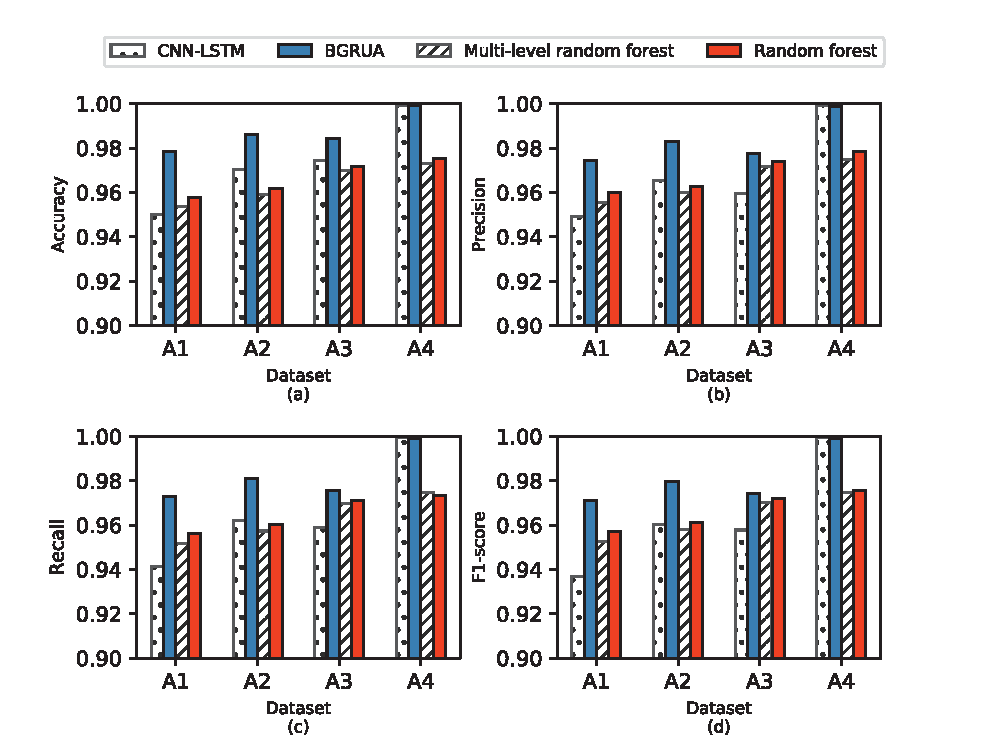
\includegraphics[width=\textwidth]{aprf.eps}
\caption{Accuracy, precision, recall, and F1-score comparisons between our model and the three baseline models.}\label{fig5}
\end{figure}




%%%%%%%%%%%%%%%%%%%%%%%%%%%%%%%%%%%%%%%%%%%%%%%%%%%%%%%%%%%%%%%%

\begin{table}[]
\caption{F1-score comparisons on Dataset A1. MRF and RF represent the multi-level random forest method and random forest method, respectively.}
\centering
\label{tab6}
\begin{tabular}{lllcc}
\hline
\textbf{Domain}      & \textbf{MRF} & \textbf{RF} & \textbf{CNN-LSTM} & \textbf{BGRUA} \\ \hline
accounts.google.com  & 0.9641 & 0.9558 & 0.9400   & 0.9935 \\
apis.google.com      & 0.6726 & 0.6156 & 0.6400   & 0.7336 \\
batr.msn.com         & 0.9261 & 0.9280 & 0.9983   & 1.0000 \\
cmg.doubleclick.net  & 0.7610 & 0.8237 & 0.9938   & 0.9927 \\
fonts.googleapis.com & 0.8590 & 0.8812 & 0.9951   & 0.9938 \\
insight.adsrvr.org   & 0.9299 & 0.9422 & 0.9666   & 0.9744 \\
s.adroll.com         & 0.8819 & 0.8657 & 0.8142   & 0.9957 \\
match.adsrvr.org     & 0.9367 & 0.9510 & 0.9653   & 0.9779 \\
www.google.com       & 0.9317 & 0.9403 & 1.0000   & 1.0000 \\
www.facebook.com     & 0.9606 & 0.9629 & 1.0000   & 0.9991 \\ \hline
\end{tabular}
\end{table}


%%%%%%%%%%%%%%%%%%%%%%%%%%%%%%%%%%%%%%%%%%%%%%%%%%%%%%%%%%%%%%%

\begin{table}[t]
\caption{F1-score comparisons on Dataset A2.}
\centering
\label{tab7}
\begin{tabular}{lllcc}
\hline
\textbf{Domain}              & \textbf{MRF}    & \textbf{RF}     & \textbf{CNN-LSTM} & \textbf{BGRUA}   \\ \hline
accounts.google.com          & 0.9509 & 0.9544 & 0.9921   & 0.9930 \\
ads.yahoo.com                & 0.9938 & 0.9959 & 1.0000   & 0.9990 \\
l.betrad.com                 & 0.9980 & 0.9988 & 0.8700   & 0.9541 \\
pagead.googlesyndication.com & 0.8718 & 0.8785 & 0.9811   & 0.9970 \\
fonts.googleapis.com         & 0.8832 & 0.8908 & 0.9942   & 0.9959 \\
ib.adnxs.com                 & 0.7543 & 0.7630 & 1.0000   & 0.9990 \\
www.livepartners.com         & 0.9914 & 0.9885 & 0.9984   & 0.9984 \\
www.googleadservices.com     & 0.9197 & 0.9305 & 0.9705   & 0.9754 \\
c.betrad.com                 & 0.9019 & 0.9065 & 0.8450   & 0.9986 \\
d.adroll.com                 & 0.9907 & 0.9923 & 0.9682   & 0.9902 \\ \hline
\end{tabular}
\end{table}




%%%%%%%%%%%%%%%%%%%%%%%%%%%%%%%%%%%%%%%%%%%%%%%%%%%%%%%%%%%%%%%%


\begin{table}[]
\centering
\caption{F1-score comparisons on Dataset A3.}
\label{tab8}
\begin{tabular}{lllcc}
\hline
\textbf{Domain}           & \textbf{MRF} & \textbf{RF} & \textbf{CNN-LSTM} & \textbf{BGRUA} \\ \hline
tpc.googlesyndication.com & 0.9168       & 0.9287      & 0.9638            & 0.9861        \\
www.google.com            & 0.9489       & 0.9463      & 1.0000            & 0.9971        \\
scontentxx.fbcdn.net      & 0.9466       & 0.9346      & 0.9425            & 0.9858        \\
d.adroll.com              & 0.9931       & 0.9939      & 1.0000            & 0.9975        \\
connect.facebook.net      & 0.9415       & 0.9345      & 0.9633            & 0.9850        \\
r.nexac.com               & 0.9966       & 0.9978      & 1.0000            & 0.9916        \\
spanalytics.yahoo.com     & 0.9929       & 0.9948      & 0.9978            & 0.9975        \\
batr.msn.com              & 0.9274       & 0.9379      & 0.9286            & 0.9979        \\
selfrepair.mozilla.org    & 0.9968       & 0.9906      & 1.0000            & 1.0000        \\
www.facebook.com          & 0.9621       & 0.9529      & 0.9994            & 0.9944        \\ \hline
\end{tabular}
\end{table}





%%%%%%%%%%%%%%%%%%%%%%%%%%%%%%%%%%%%%%%%%%%%%%%%%%%%%%%%%%%%%%


\begin{table}[]
\caption{F1-score comparisons on Dataset A4.}
\centering
\label{tab9}
\begin{tabular}{lllcc}
\hline
\textbf{Domain}      & \textbf{MRF} & \textbf{RF} & \textbf{CNN-LSTM} & \textbf{BGRUA} \\ \hline
beacon.krxd.net      & 0.9934       & 0.9943      & 0.9975            & 0.9983        \\
secure.adnxs.com     & 0.9088       & 0.9212      & 0.9996            & 0.9997        \\
www.google.com       & 0.8582       & 0.8526      & 0.9987            & 0.9992        \\
www.facebook.com     & 0.9633       & 0.9622      & 1.0000            & 1.0000        \\
pixel.quantserve.com & 0.9990       & 0.9995      & 1.0000            & 1.0000        \\
ib.adnxs.com         & 0.7483       & 0.7685      & 0.9989            & 0.9991        \\
d.adroll.com         & 0.9960       & 0.9962      & 1.0000            & 1.0000        \\
tags.tiqcdn.com      & 0.9869       & 0.9871      & 0.9991            & 0.9989        \\
bat.bing.com         & 0.9935       & 0.9935      & 1.0000            & 1.0000        \\
assets.adobedtm.com  & 0.9857       & 0.9857      & 1.0000            & 1.0000        \\ \hline
\end{tabular}
\end{table}





%%%%%%%%%%%%%%%%%%%%%%%%%%%%%%%%%%%%%%%%%%%%%%%%%%%%%%%%%%%%%%%


\begin{figure}[]
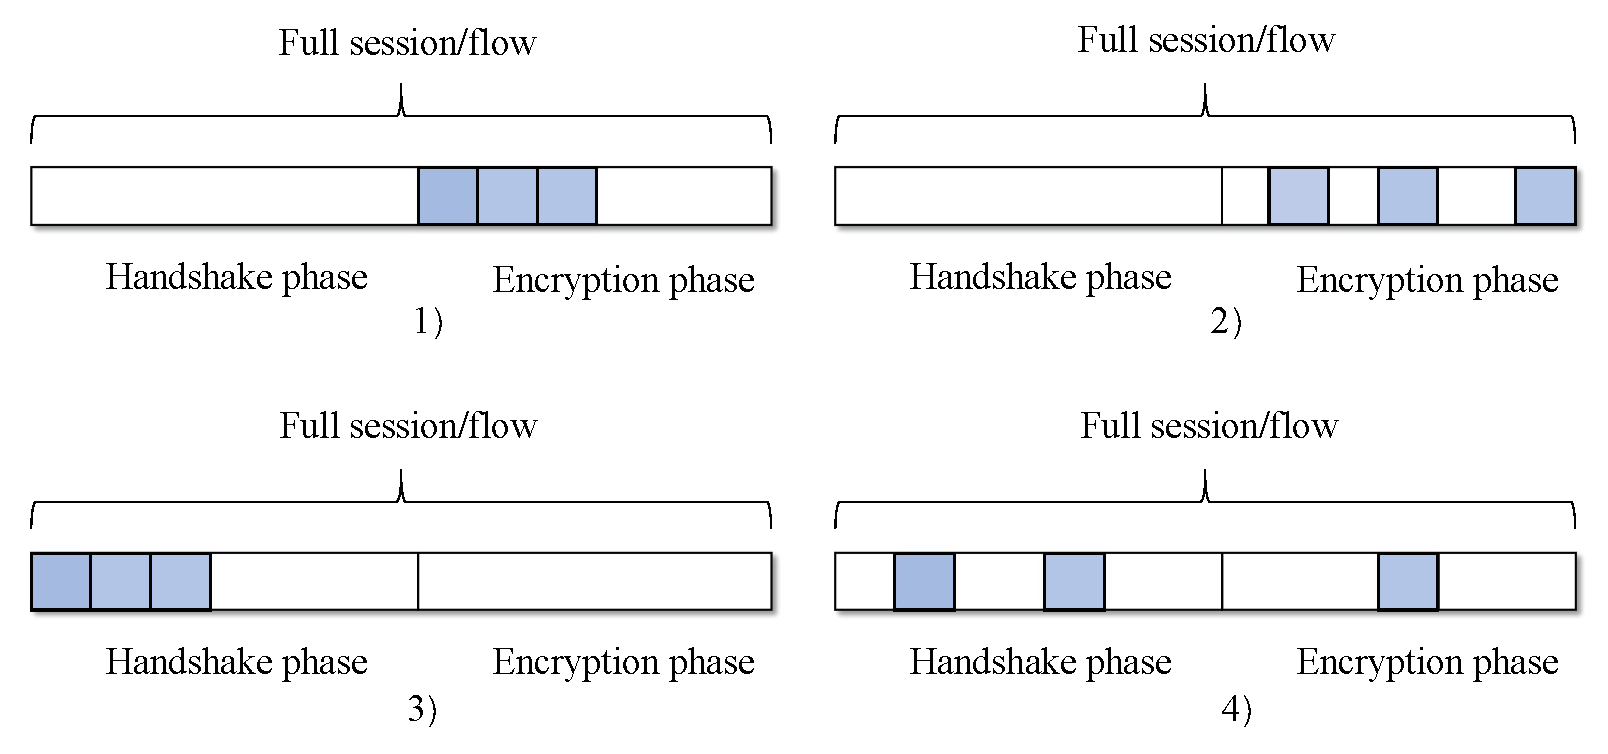
\includegraphics[width=\textwidth]{pktloc.eps}
\caption{Overview of packet locations in a flow or session. 1) The first three packets in the encryption phase, 2) a random selection of three packets in the encryption phase, 3) the first three packets in the full session, and 4) any three packets at random locations.}\label{fig6}
\end{figure}

As shown in Figure~\ref{fig6}, to explore the effects of different packet locations within a flow or session as the inputs for our model, we selected packets in four ways: 1) the first three packets in the encryption phase, 2) any three packets in the encryption phase, 3) the first three packets in the full session, and 4) any three packets at random locations. As shown in Figure \ref{fig7}, the accuracy of the proposed model using the first three packets in a full session as inputs is 99\%, which is more than 10\% higher than that when using the first three packets in the encryption phase. This is mainly because the first three packets in a session are in the handshake phase of the TLS connection. In this phase, the client and server exchange distinguishable features, such as protocol versions, encryption methods, and compression methods.
%***provide a few example features***. 
However, in the phase of encrypted data transmission, packet payloads are completely irregular based on encryption. For encrypted data, our model can also effectively mine features and achieve an accuracy of 88\%. Randomly selecting three packets in a full session results in an accuracy of 92\%, where packets in the handshake phase account for 53\%. These experimental results demonstrate that the handshake phase of a flow or session prior to encrypted transmission has a significant impact on the performance of traffic classification.



Furthermore, we conducted experiments on Dataset A4 to explore the effects of different hyperparameters on the performance of BGRUA, including $U$, $B$, and $P$. $U$ represents the hidden units of the bidirectional GRU layer, $P$ denotes the first $P$ packets selected in a session, and $B$ is the number of bytes in each packet. By default, we use the following parameter values: $U = 256$, $B = 900$, and $P = 3$. For each experiment, we only changed one parameter and used the default values for the other parameters. As shown in Figure~\ref{fig8}(a), the performance of our model is sensitive to the value of $U$. When $U$ is 64, our model achieves an accuracy of approximately 99\%, which is 6\% higher than the case with $U = 8$. This is mainly because $U$ implicitly determines the memory capacity of the GRU. In practice, it is extremely important to assign an appropriate value for $U$.
As shown in Figure~\ref{fig8}(b), the accuracy of our model reaches 98\% when the parameter $B$ is equal to 225. After increasing the value of $B$ to 900, accuracy increases by 1\%. This indicates that although the first 225 bytes carry sufficient information, the best results can be achieved by using 900 bytes for HTTPS traffic classification. In Fig.~\ref{fig8}(c), there is a dramatic increase in accuracy when the number of packets increases from one to two. Other metrics exhibit similar trends, indicating that at least two packets should be selected in practice.


\begin{figure}[]
\centering
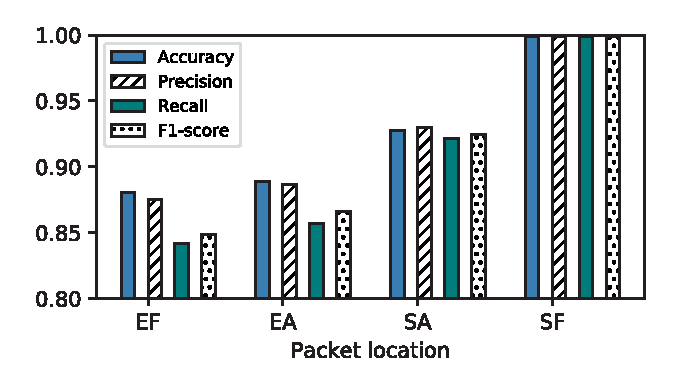
\includegraphics[width=\textwidth]{EF.eps}
\caption{Effects of different packet locations selected in a flow or session on the performance of our model. EF and EA represent the first three and random three packets in the encryption phase. SF and SA denote the first three and random three packets in a full session.}\label{fig7}
\end{figure}


% ***need describe subfigures (a)*** (b)***, and (c)***

\begin{figure}[]
\centering
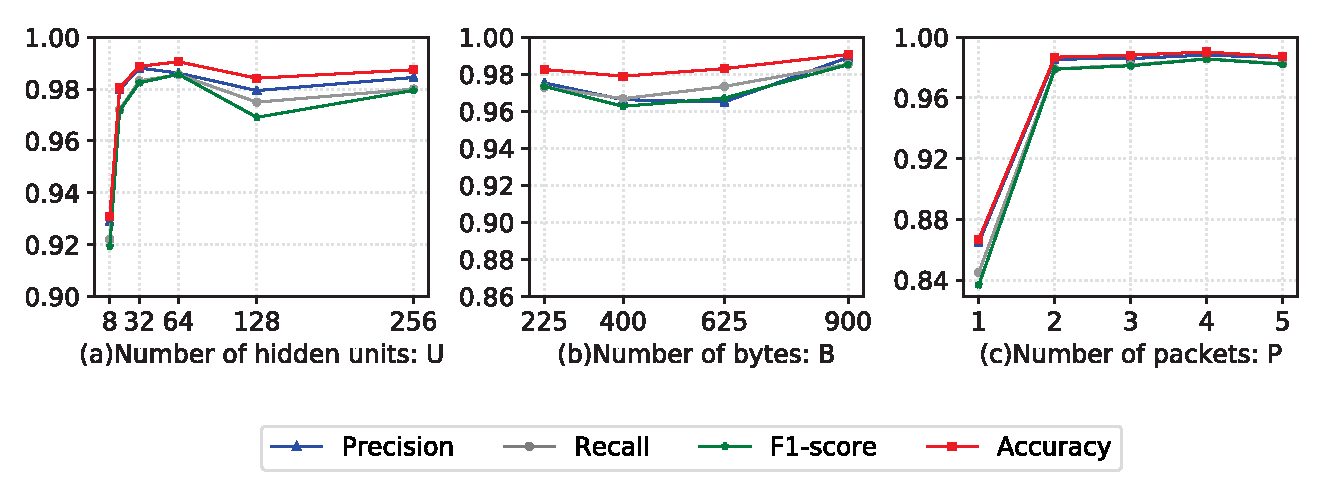
\includegraphics[width=\textwidth]{hyperpara.eps}
\caption{Effects of different hyperparameters values on experimental results.}\label{fig8}
\end{figure}

Model complexity is another important metric for evaluating the performance of our proposed model. 
Table~\ref{tab10} lists the main parameters of each layer in BGRUA. As discussed in Section \ref{sec: bidirectional_gru_layer}, the first two layers are constructed by stacking two basic bidirectional GRU cells. The 18 vectors with 150 dimensions form an $18 \times 150$ tensor that is fed into GRU layer-1, which contains 256 hidden units. The output (i.e., an $18 \times 256$ tensor) is sent to GRU layer-2, which has the same structure as GRU layer-1. The output of GRU layer-2 is weighted and summed by the attention layer and sent to the dense layer to undergo fully connected operations. Table~\ref{tab11} compares the time consumption and parameters between the CNN-LSTM and BGRUA models.
The average training and testing times in Table~\ref{tab11} represent datasets A1 to A4. These experimental results demonstrate that the number of parameters in our BGRUA model is reduced by more than seven times compared to the CNN-LSTM model. Additionally, overall training time is reduced by approximately 11 times and testing time is reduced by approximately six times. These results indicate that the time consumption of classification is proportional to the number of parameters. Therefore, reducing the complexity of model parameters can improve the speed of classification.
%The time consumption of the model can be reduced by optimizing parameters.


%***The above paragraph needs more fine-grained description and analysis.***

\begin{table}[]
\caption{Detailed parameters of the proposed BGRUA model.}
\centering
\begin{tabular}{cccc}
\hline
\multicolumn{1}{c|}{\textbf{Layer}}   & \multicolumn{1}{c|}{\textbf{Input Shape}} & \multicolumn{1}{c|}{\textbf{Output Shape}} & \textbf{Weight} \\ \hline
\multicolumn{1}{c|}{GRU Layer-1} & \multicolumn{1}{c|}{(18, 150)}            & \multicolumn{1}{c|}{(18, 256)}             & 214272          \\ \hline
\multicolumn{1}{c|}{GRU Layer-2} & \multicolumn{1}{c|}{(18, 256)}            & \multicolumn{1}{c|}{(18, 256)}             & 295680          \\ \hline
\multicolumn{1}{c|}{Attention}        & \multicolumn{1}{c|}{(18, 256)}            & \multicolumn{1}{c|}{256}                   & 274             \\ \hline
\multicolumn{1}{c|}{Dense}            & \multicolumn{1}{c|}{256}                  & \multicolumn{1}{c|}{13}                    & 3341            \\ \hline
Total weights                         & 513,567                                   &                                            &                 \\ \hline
\end{tabular}
\label{tab10}
\end{table}


\begin{table}[]
\caption{Time consumption of models}
\centering
\begin{tabular}{c|c|c|c}
\hline
\textbf{Model} & \textbf{Parameters} & \textbf{Training time/epoch} & \textbf{Testing time} \\ \hline
CNN-LSTM            & 3754k            &                    
188.58 ms   &         10s           \\ \hline
BGRUA                & 514k             &                      17.24ms     &         1.6s          \\ \hline
\end{tabular}

\label{tab11}
\end{table}


\subsubsection{Model Comparison on Dataset B}
Regarding Dataset B, we only compared BGRUA to CNN-LSTM because the random forest algorithms require features in two directions. For detailed analysis, we have plotted heatmaps of the confusion matrices of BGRUA and CNN-LSTM in Figures~\ref{fig9}(a) and \ref{fig9}(b), respectively. 
One can see that the 11 classes on the diagonal exhibit a deeper blue color, demonstrating the effective classification performance of both models for HTTPS services. It is worth noting that the lightest blue colors on the diagonal indicate that both models tend to misjudge the classes of ``pos.baidu.com", ``pan.baidu.com," and ``www.baidu.com." This is because these three classes belong to the same service provider. Similar patterns of services from the same provider can easily confuse classifiers.


\begin{figure}[htbp]
\centering
\begin{minipage}[t]{0.48\textwidth}
\centering
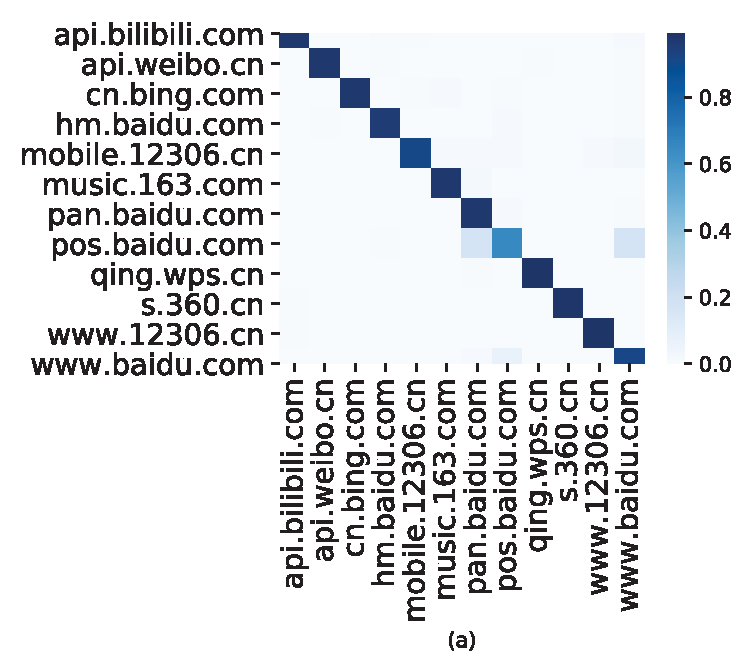
\includegraphics[width=6cm]{heatmap-bgrua.eps}
\end{minipage}
\begin{minipage}[t]{0.48\textwidth}
\centering
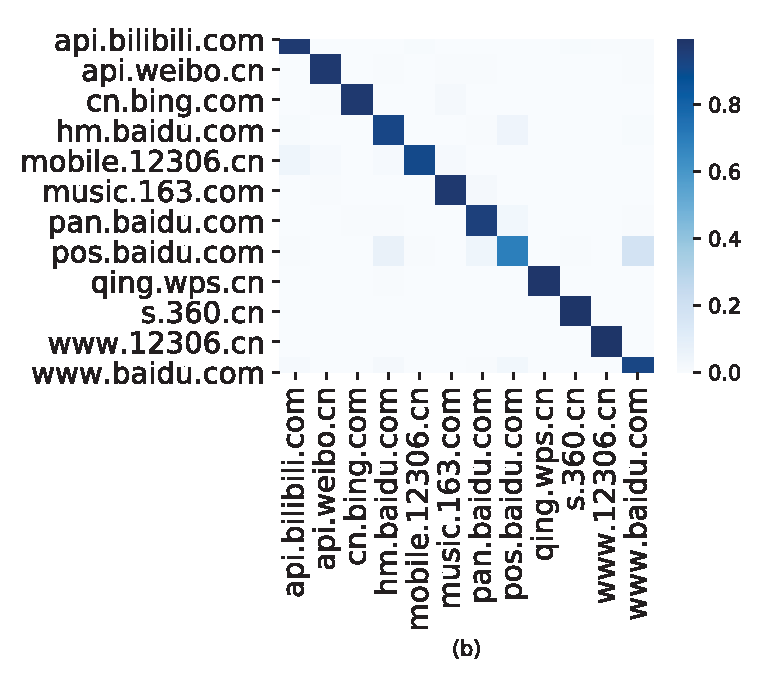
\includegraphics[width=6cm]{heatmap-cnn.eps}
\end{minipage}
\caption{Comparison of BGRUA and CNN-LSTM. Parts (a) and (b) represent the confusion matrices of BGRUA and CNN-LSTM, respectively.}\label{fig9} 
\end{figure}



Figure~\ref{fig10} contains three subgraphs presenting the precision, recall, and F1-score values for 12 classes in Dataset B. In Figure~\ref{fig10}(a), the precision values for 10 classes are greater than 90\% and the average precision of our BGRUA model is greater than that of the CNN-LSTM model by as much as 2.51\%. As shown in Fig.~\ref{fig10}(b), for the class of ``pos.baidu.com," BGRUA achieves a recall of 80\%, representing an improvement of 11\% compared to CNN-LSTM. In Figure~\ref{fig10}(c), among all 12 classes of HTTPS traffic, the F1-scores of four classes for our model are greater than those for the CNN-LSTM model. There are six classes whose F1-scores are approximately equal. Both models perform poorly on the ``pos.baidu.com" class and unsatisfactorily on the ``mobile.12306.cn" class. This dataset contains multiple services from the same service provider (e.g., four types of traffic from ``baidu" and two from ``12306"). Because this flow-based dataset only contains traffic from clients to servers, the information carried by the clients is insufficient for distinguishing various services from the same service provider. However, for services from different service providers, our model can achieve excellent performance. These experimental results demonstrate that it is better to consider full sessions to differentiate services from the same service provider.




% ***need subfigure indicator (a)***(b)***(c)***
\begin{figure}[]
\centering
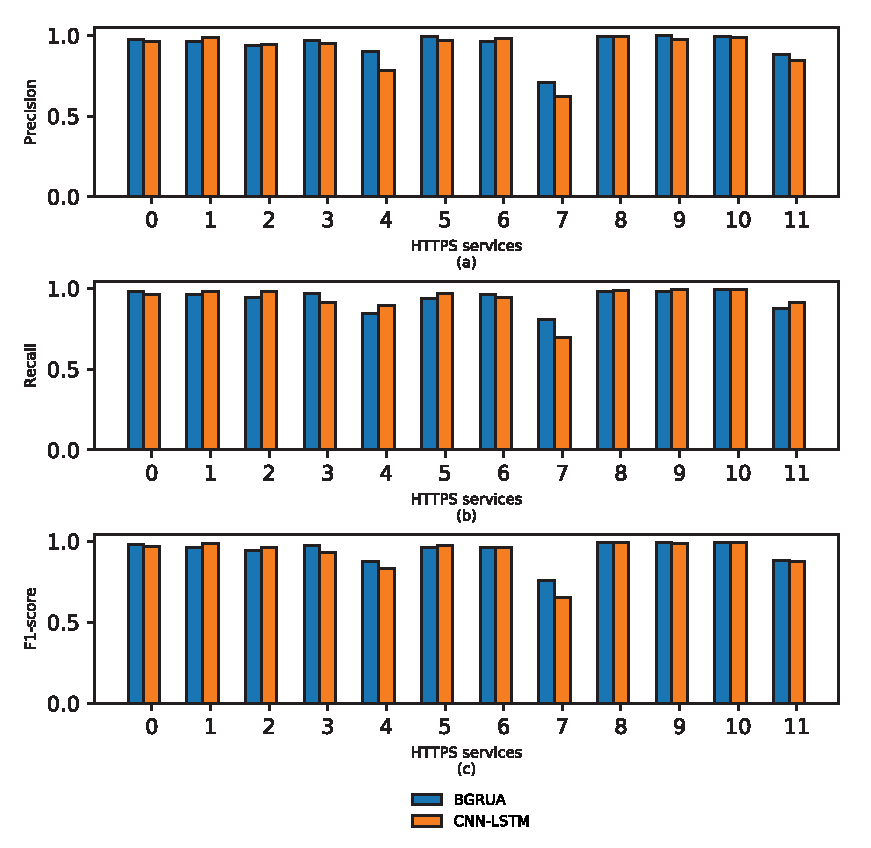
\includegraphics[width=\textwidth]{histogram.eps}
\caption{Comparison between our model and CNN-LSTM. The values of 0 to 11 on the x axis represent the classes of ``api.bilibili.com," ``api.weibo.cn," ``cn.bing.com," ``hm.baidu.com," ``mobile.12306.cn," ``music.163.com," ``pan.baidu.com," ``pos.baidu.com," ``qing.wps.cn," ``s.360.cn," ``www.12306.cn," and ``www.baidu.com," respectively.}\label{fig10}
\end{figure}

\begin{figure}[t]
\centering
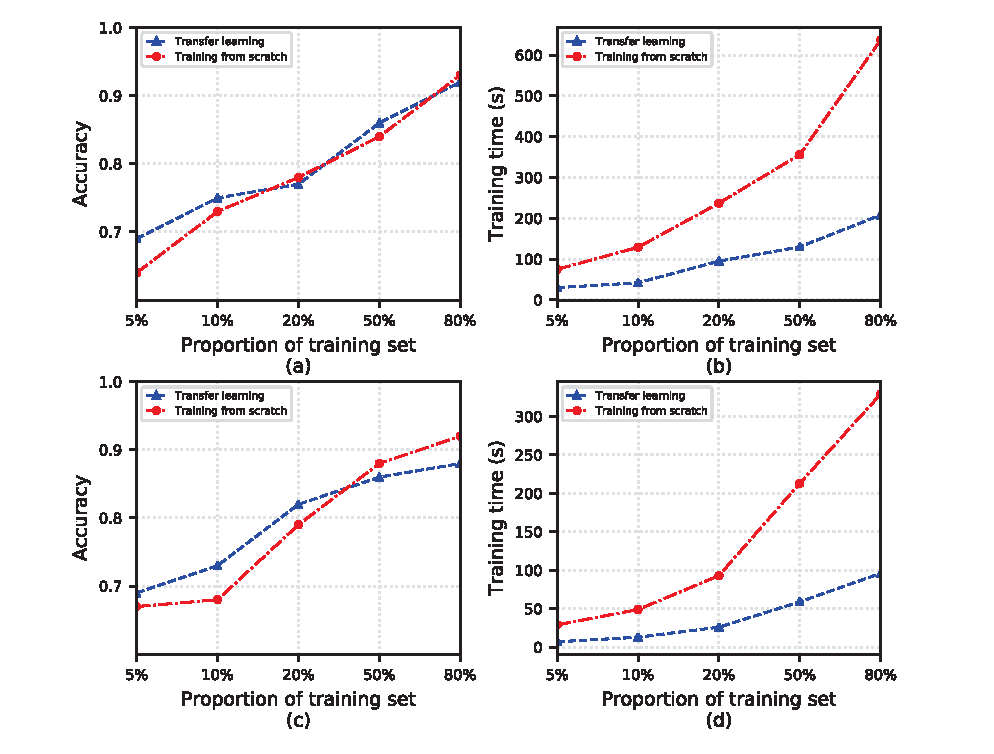
\includegraphics[width=\textwidth]{transfer.eps}
\caption{Evaluation of transfer learning. Parts (a) and (b) represent the changes in accuracy and training time, respectively, with increasing amounts of training data.}\label{fig11}
\end{figure}



\subsubsection{Effects of transfer learning} 
First, a source model was trained on Dataset A4. Two groups of traffic were then selected from Dataset C to evaluate the effects of transfer learning by retraining the source model. The first group contained 13 categories that were the same as the traffic categories in Dataset A4. The second group contained six categories that were different from Dataset A4. We conducted five experiments with new training data accounting for 5\%, 10\%, 20\%, 50\%, and 80\% of the total data. The experimental results for the first group of data are presented in Figures~\ref{fig11}(a) and \ref{fig11}(b). These figures present the effects of the number of training samples on the accuracy and training speed of the model, respectively. 
Overall, the model based on transfer learning has higher accuracy and faster training speed. When the proportion of training data is relatively small (i.e., 5\%), the accuracy of the fine-tuned model is 5\% higher than that of the model trained from scratch. This is because when the number of training samples is small, the features in the training data are insufficient to represent the real data distribution. Using relevant prior knowledge to help learn new knowledge can compensate for this shortcoming. Furthermore, for new learning tasks, the convergence speed of the model is significantly increased by transfer learning. As shown in Figure~\ref{fig11}(a), in the cases with few training samples, the week generalization ability of the model trained from scratch results in lower accuracy. In contrast, transfer learning can use existing knowledge to assist in training, resulting in significantly improved accuracy. When the proportion of training samples is relatively large, the gap between the two training methods shrinks because the learning ability of the model trained from scratch increases. 

Evaluations of the second group are presented in Figures~\ref{fig11}(c) and \ref{fig11}(d). These figures exhibit similar trends compared to Figures~\ref{fig11}(a) and \ref{fig11}(b). In Figure~\ref{fig11}(c), the accuracy of the transfer learning approach is greater than that of training from scratch. This is because some new HTTPS services samples are used that were not considered in the source model. When the proportion of training samples increases, the results of training from scratch exhibit greater accuracy. However, training time consumption increases much more compared to the transfer learning method. For traffic that is not included in the source dataset, the model based on transfer learning exhibits excellent performance and efficiency, further demonstrating the effectiveness of our method.



\section{Conclusions}
Encrypted HTTPS traffic has introduced new challenges into network management and security analysis. In this paper, we proposed a novel model based on bidirectional GRUs and an attention mechanism to classify encrypted HTTPS traffic automatically. Extensive experimental results demonstrated that our model outperforms three state-of-the-art models. This confirms that our model is more suitable for the classification of HTTPS traffic. One of the most significant findings of this study is that deep learning methods perform more stably than traditional machine learning methods. This is mainly because the time-related features adopted in the traditional methods are susceptible to changes in network environments, which affects classification performance. Fluctuations in accuracy caused by changes in packet locations proved that the TLS negotiation phase has a significant impact on the performance of traffic classification. We analyzed the sensitivity of the proposed BGRUA model to different hyperparameters and obtained a set of reasonable values experimentally. To achieve optimal results, hyperparameters must be strictly controlled in practice. Furthermore, comparative experiments between session-based and flow-based datasets revealed that bidirectional HTTPS traffic contains richer features, which can distinguish various services from the same service provider more accurately. Additionally, we introduced the concept of transfer learning into encrypted traffic classification. Experimental results demonstrated that training speed on new datasets is significantly improved by transfer learning.

\normalem
\bibliography{INS_15456}
\bibliographystyle{unsrt}

\end{document}




